\subsection[Architektura środowiska testowego]{Architektura środowiska testowego}
\begin{figure}[H]
    \centering
    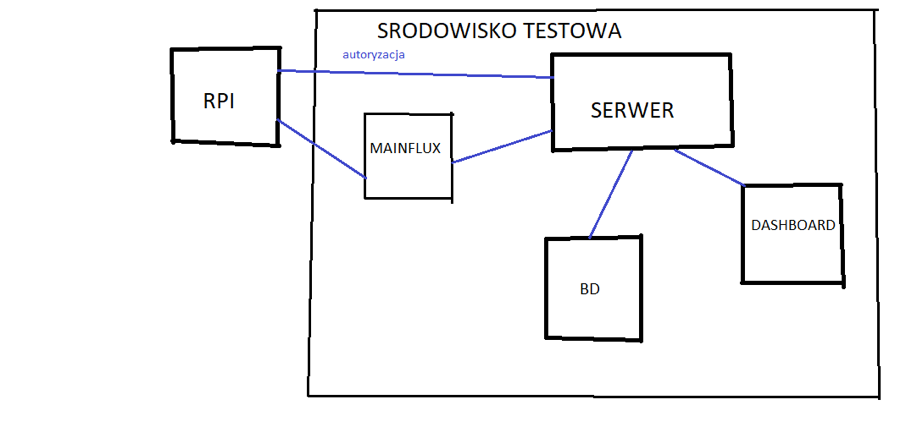
\includegraphics[width=\textwidth]{kp01}
    \caption{Schemat przedstawiający podstawowe zależności w środowisku testowym } % role Środowiska testowego w dedykowanym systemie
    \label{fig:iotarch}
\end{figure} 
Środowisko testowe składa się z kilku komponentów: serwera, platformy Mainflux, bazy danych oraz dashboardu. Wszystkie wymienione elementy znajdują się na jednej maszynie.
Serwer to oprogramowanie, które ma kilka zadań do spełnienia, pierwszym jest zapewnienie autoryzacji platformy wykonującej. Każda platforma jest skonfigurowana w Mainfluxie jako \textit{rzecz} (rozdział~\ref{subsection:wp}), która posiada swój zewnętrzny identyfikator oraz klucz, w momencie, gdy platforma wykonująca chce otrzymać swoje dane (tzn. klucz rzeczy, identyfikator rzeczy oraz 2 przypisane kanały) wysyła żądanie HTTP na serwer z zewnętrznym identyfikatorem oraz kluczem. Platforma wykonująca potrzebuje 2. kanałów, ponieważ na jednym będzie wysyłała wiadomości, a na drugim odbierała. Serwer po otrzymaniu zapytania sprawdza czy zewnętrzny identyfikator przesłany przez platformę wykonującą znajduję się już w bazie danych, jeśli tak to pobiera jego dane oraz zwraca je. W przeciwnym razie serwer dzięki Mainflux CLI loguje się jako administrator, tworzy nową rzecz oraz 2 kanały, po czym przypisuje je do stworzonej rzeczy oraz do rzeczy serwera. Rzecz serwera jest to utworzony obiekt przy starcie środowiska testowego, który ma przypisane do siebie wszystkie kanały. 
Kolejnym zadaniem serwera jest przesyłanie wiadomości z panelu użytkownika na platformę wykonującą oraz odbieranie wiadomości od platformy wykonującej. Wysyłanie wiadomości jest stosunkowo łatwe. Wystarczy, że serwer wyśle payload na odpowiedni kanał, który nasłuchuje w tym samym czasie. Z kolei odbieranie wiadomości jest bardziej skomplikowane, aby odebrać wiadomość serwer musi nasłuchiwać na kanale. Ze względu na to, że wiele platform wykonujących może w tym samym momencie wysyłać wiadomości, środowisko testowe powinno jednocześnie nasłuchiwać na wszystkich kanałach. Serwer dodaje kanały które znajdują się w bazie danych. Oznacza to, że w momencie gdy nowa platforma wykonująca przechodzi proces autoryzacji, serwer musi automatycznie odświeżyć listę kanałów, które nasłuchują na przesłaną wiadomości.
\begin{figure}[H]
    \centering
    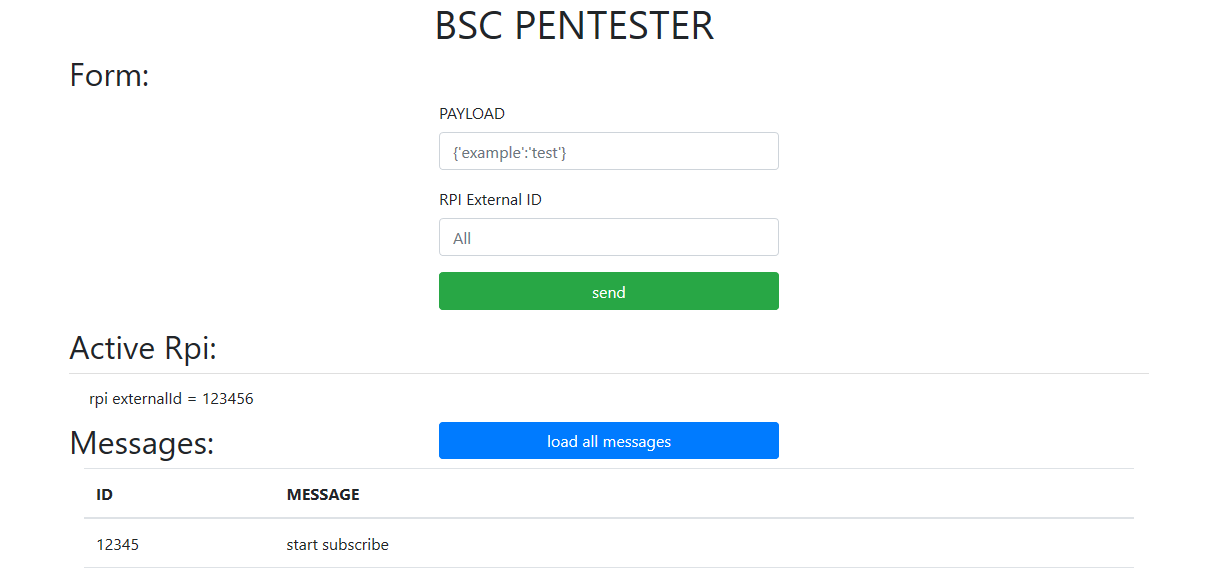
\includegraphics[width=\textwidth]{kp09}
    \caption{Zrzut ekranu - interfejs pentestera}
    \label{fig:dahsboard}
\end{figure}
Środowisko oferuje rest api, które pozwoli na udostępnienie metod potrzebnych do stworzenia Dashboardu. Dashboard jest to łatwy w odczycie interfejs, który pośredniczy miedzy pentesterem a serwerem. Jednym z celów rest api jest umożliwienie pobrania wiadomości, jakie serwer odebrał. Pozwala to pentesterowi na przeglądanie wiadomości. Kolejna metoda ma za zadanie zwrócić listę aktywnych platform wykonujących. Ta lista znajduje się na serwerze oraz jest uaktualniana co 5 sekund. Uaktualnianie polega na tym, że platforma wykonująca co 2s zgłasza aktywność, jeśli serwer nie otrzyma wiadomości od platformy przez więcej niż 4s aktualny wynik zostaje usunięty. Następną udostępnioną metodą jest wysłanie ładunku na platformę wykonującą. Serwer pozwala na wysłanie wiadomości na wskazaną platformę lub do wszystkich aktywnych urządzeń. Aby pentester mógł wysłać payload na pojedynczą platformę, musi wpisać zewnętrzny identyfikator urządzenia. Serwer, który otrzyma zapytanie z takim identyfikatorem sprawdza, czy wskazane urządzenie istnieje, jeśli tak to pobiera jego kanał, na którym nasłuchuje oraz wysyła wiadomość. Odpowiedź pentester będzie mógł przeczytać na liście przesłanych wiadomości.
Opisane ST zostało wykorzystane do zapewnienia pentesterowi stałego doestępu do platform wykonujących oraz zdalnego wykonywania testów. Sposób użycia ST został przedstawiony w scenariuszach \textit{Podszywanie pod HID}, \textit{Pharming} i \textit{Mitm} (rozdziały~\ref{sce:klawiatura}, \ref{sce:phar} i~\ref{sce:mitm}).